%%%%%%%%%%%%%%%%%%%%%%%%%%%%%%%%%%%%%%%%%%%%%%%%%%%%%%
% A Beamer template for University of Wollongong     %
% Based on THU beamer theme                          %
% Author: Qiuyu Lu                                   %
% Date: July 2024                                    %
% LPPL Licensed.                                     %
%%%%%%%%%%%%%%%%%%%%%%%%%%%%%%%%%%%%%%%%%%%%%%%%%%%%%%
% Customized for Sharif University of Technology     %
%%%%%%%%%%%%%%%%%%%%%%%%%%%%%%%%%%%%%%%%%%%%%%%%%%%%%%


\documentclass[aspectratio=169]{beamer}
\usefonttheme{serif}
%\documentclass[serif]{beamer}  % for 4:3 ratio
\usepackage[T1]{fontenc} 
\usepackage{fourier} % see "http://faq.ktug.org/wiki/uploads/MathFonts.pdf" for other options
\usepackage{hyperref}
\usepackage{latexsym,amsmath,xcolor,multicol,booktabs,calligra}
\usepackage{graphicx,pstricks,listings,stackengine}
\usepackage{lipsum}
\usepackage{tikz}
\usepackage{svg}
\usepackage{amsmath}
\usepackage{amssymb}
\usepackage{graphicx}

\author{Ali Sharifi-Zarchi}
\title{Machine Learning (CE 477)}
\subtitle{Fall 2024}
\institute{
    CE Department \\
    Sharif University of Technology
}
%\date{\small \today}
% \usepackage{UoWstyle}
\usepackage{SUTstyle}

% defs
\def\cmd#1{\texttt{\color{red}\footnotesize $\backslash$#1}}
\def\env#1{\texttt{\color{blue}\footnotesize #1}}
\definecolor{deepblue}{rgb}{0,0,0.5}
\definecolor{deepred}{RGB}{153,0,0}
\definecolor{deepgreen}{rgb}{0,0.5,0}
\definecolor{halfgray}{gray}{0.55}

\lstset{
    basicstyle=\ttfamily\small,
    keywordstyle=\bfseries\color{deepblue},
    emphstyle=\ttfamily\color{deepred},    % Custom highlighting style
    stringstyle=\color{deepgreen},
    numbers=left,
    numberstyle=\small\color{halfgray},
    rulesepcolor=\color{red!20!green!20!blue!20},
    frame=shadowbox,
}


\begin{document}

\begin{frame}
    \titlepage
    \vspace*{-0.6cm}
    \begin{figure}[htpb]
        \begin{center}
            
\includegraphics[keepaspectratio, scale=0.25]{pic/sharif-main-logo.png}
        \end{center}
    \end{figure}
\end{frame}
\begin{frame}    
\tableofcontents[sectionstyle=show,
subsectionstyle=show/shaded/hide,
subsubsectionstyle=show/shaded/hide]
\end{frame}

\section{Introduction}

\begin{frame}{Recap: Self-Attention Mechanism}

\textbf{Inputs:}\\
Input vectors: $\mathbf{x}$ (shape: $N \times D$)

\vspace{0.5cm}

\textbf{Operations:}
\begin{align*}
\text{Key vectors:} & \quad \mathbf{k} = \mathbf{W}_K^T \mathbf{x} \\
\text{Value vectors:} & \quad \mathbf{v} = \mathbf{W}_V^T \mathbf{x} \\
\text{Query vectors:} & \quad \mathbf{q} = \mathbf{W}_Q^T \mathbf{x} \\
\text{Alignment:} & \quad e_{i,j} = \frac{\mathbf{q}_j \cdot \mathbf{k}_i}{\sqrt{D}} \\
\text{Attention:} & \quad a = \text{softmax}(e) \\
\text{Output:} & \quad \mathbf{y}_j = \sum_i a_{i,j} \mathbf{v}_i
\end{align*}

\vspace{0.5cm}

\textbf{Outputs:}\\
Context vectors: $\mathbf{y}$ (shape: $D_o$)

\vspace{0.5cm}

\textbf{Diagram of Self-Attention:}


\end{frame}

\begin{frame}{}
    \begin{itemize}%[<+-| alert@+>] % stepwise alerts
        \item Self-attention-based architectures, in particular Transformers, have become the model of choice in natural language processing (NLP).
        \item The dominant approach is to pre-train on a large text corpus and then fine-tune on a smaller task-specific dataset.
        \item In computer vision, however, convolutional architectures remain dominant.
    \end{itemize}
\end{frame}

\begin{frame}{Strengths of CNNs}
    \begin{itemize}
        \item \emph{Local Feature Extraction:} CNNs excel at extracting local patterns through convolutions, detecting edges, textures, and shapes in a hierarchical manner.
        \item \emph{Translation Invariance:} The use of convolution and pooling layers helps CNNs detect features regardless of their position in the image.
        \item \emph{Efficient Computation:} Weight sharing in convolutional layers makes CNNs computationally efficient compared to fully connected networks for images.
    \end{itemize}
\end{frame}

\begin{frame}{Limitations of CNNs}
    \begin{itemize}
        \item \emph{Limited Receptive Field:} Early convolutional layers only see a small portion of the image at a time (local features), while later layers expand the receptive field, but still require deep architectures to model long-range dependencies.
        \item \emph{Pooling Information Loss:} Pooling layers (e.g., max-pooling) help reduce computational costs but can lose important spatial details, especially for global image understanding.
        \item \emph{Struggle with Global Context:} CNNs focus more on local spatial hierarchies and have difficulty capturing global relationships between distant parts of an image.
    \end{itemize}
\end{frame}

\begin{frame}{CNNs Struggle with Global Context}
    \begin{itemize}
        \item Why it matters: For tasks that require understanding the entire image (e.g., image classification, where the relationship between distant parts of the image may be important), CNNs often require deep architectures to get the full picture.
        \item Feature Hierarchy: CNNs build a hierarchical structure of features but rely on many layers to achieve global understanding, leading to more complexity.
    \end{itemize}
\end{frame}



\section{Transformers for Vision}

\begin{frame}{Transformers: From Language to Vision}
    \begin{itemize}
        \item The Transformer architecture was designed for \textbf{sequence-to-sequence learning}.
        \item Transformers have revolutionized NLP and become the model of choice.
        % \item In the field of \textbf{Computer Vision} however, the dominant architecture has remained the CNN.
	\item Is it possible to adapt the Transformer for image data?
    \end{itemize}
\end{frame}


\begin{frame}{Idea \#1: Add Attention to Existing CNNs}
    \begin{itemize}
        \item Model is still a CNN!
    \end{itemize}
    \begin{figure}
        \centering
        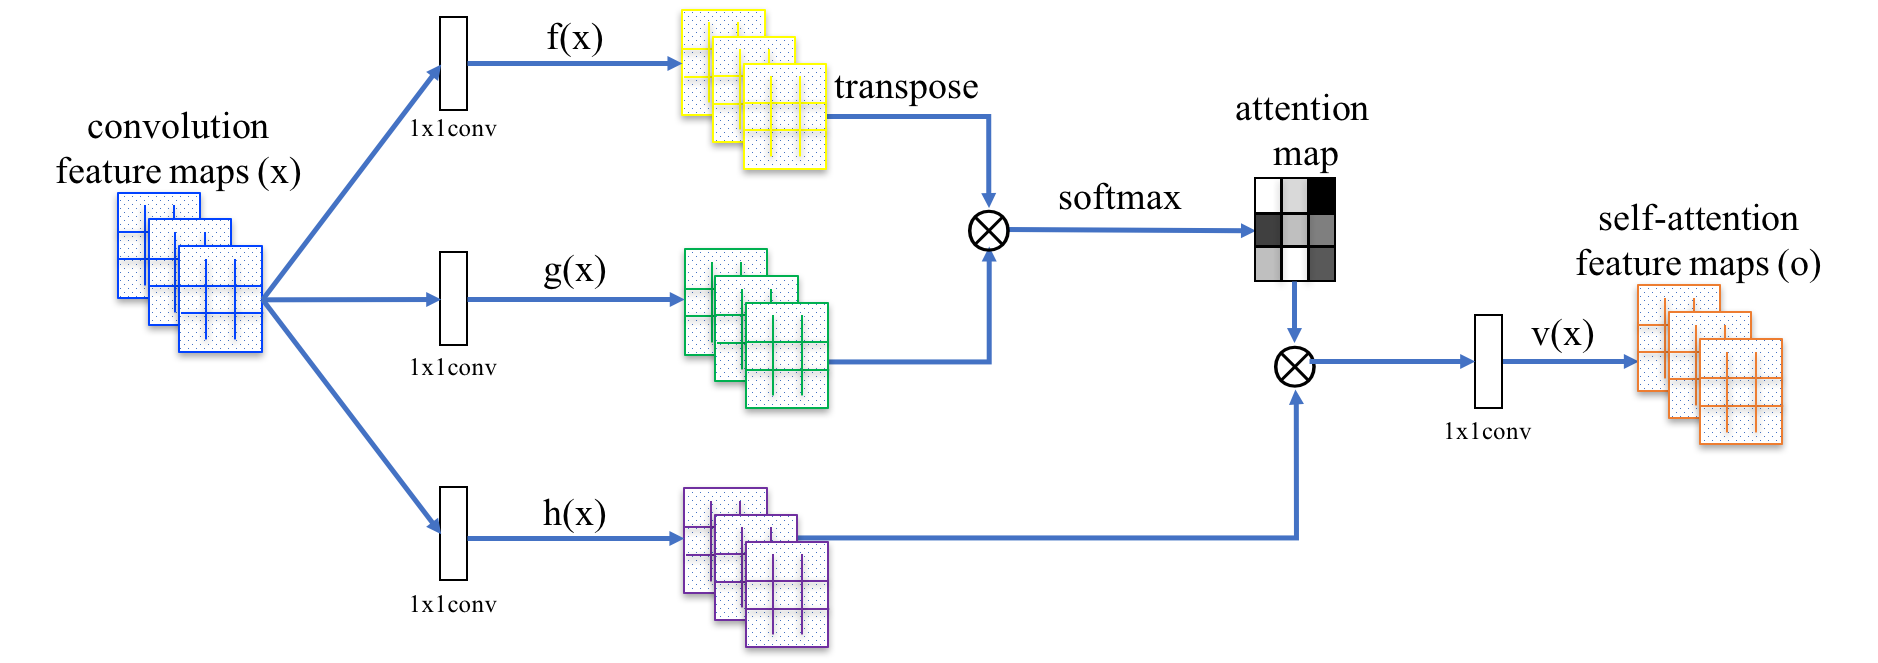
\includegraphics[width=\linewidth]{pic/framework}
        % \caption{Add Self-Attention blocks between existing ResNet blocks.}
        \label{fig:idea1}
    \end{figure}
\end{frame}

\begin{frame}{Idea \#2: Replace Convolution with “Local Attention”}
    \begin{itemize}
        \item Lots of tricky details, hard to implement, only marginally better than ResNets.
    \end{itemize}
    \begin{figure}
        \centering
        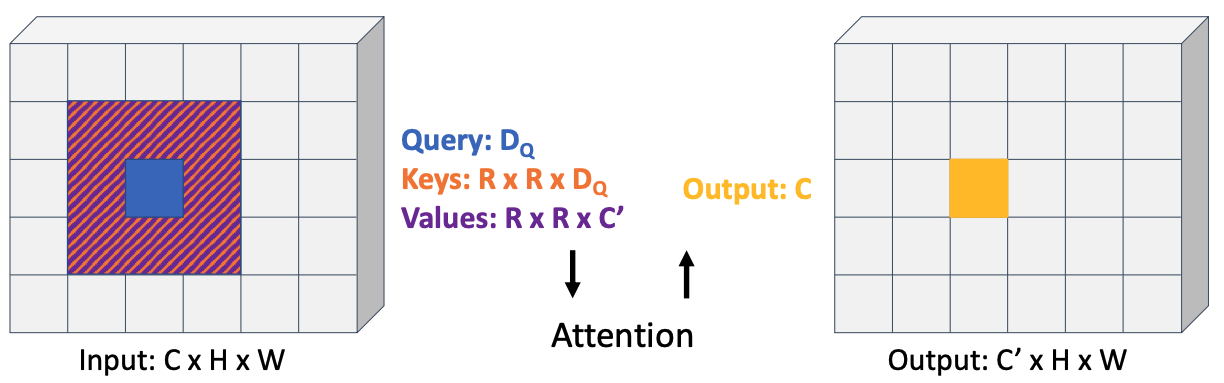
\includegraphics[width=\linewidth]{pic/idea2}
        % \caption{Replace all convolutional layers in CNNs with local attention.}
        \label{fig:idea1}
    \end{figure}
\end{frame}


\begin{frame}{Idea \#3: Standard Transformers on Pixels}
    \begin{itemize}
        \item Insane memory usage!
    \end{itemize}
    \begin{figure}
        \centering
        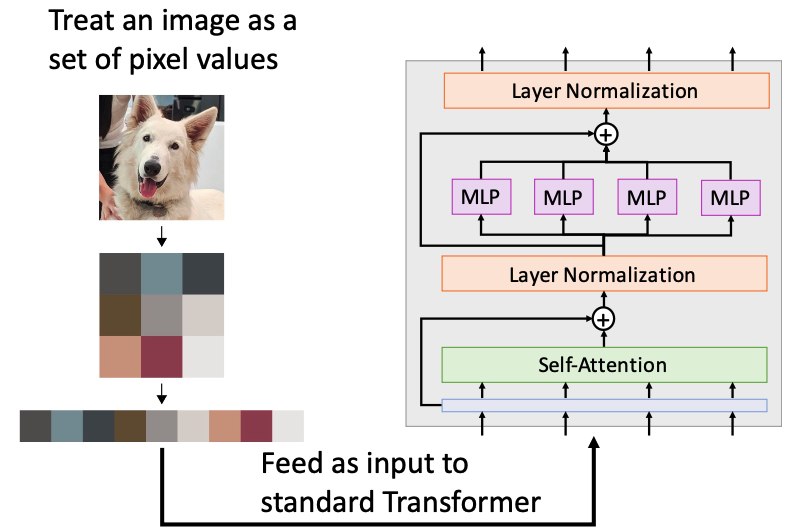
\includegraphics[width=0.5\linewidth]{pic/idea3}
        % \caption{Treat each image pixel as an input token for the transformer.}
        \label{fig:idea1}
    \end{figure}
\end{frame}


\begin{frame}{Idea \#4: Standard Transformer on Patches}
    \begin{itemize}
        % \item Follow the original Transformer as closely as possible.
        \item Fixes idea \#1 by entirely replacing convolutional layers.
        \item Fixes idea \#2 by simplifying implementation.
        \item Fixes idea \#3 by reducing memory usage.
        \item This is the main idea behind \textbf{Vision Transformers}!
    \end{itemize}
\end{frame}


\section{Vision Transformers}

\begin{frame}{Processing Text}
    \begin{itemize}
        \item \textbf{Token Embeddings}: The input text is broken down into individual tokens. 
	\item \textbf{Word Embeddings}: Each token is converted into a fixed-length vector representation.
	\item \textbf{Self-Attention on Tokens}: The transformer's self-attention mechanism is applied to these word embeddings. 
    \end{itemize}
\end{frame}

\begin{frame}{Processing Images}
    \begin{itemize}
        \item \textbf{Patch Embeddings}: ViT splits an image into fixed-size patches (e.g., $16\times16$ pixels). Each patch is treated like a token in NLP, much like words in a sentence.
	\item \textbf{Linear Embedding}: Each patch is flattened into a 1D vector and then linearly projected to a fixed-length embedding.
	\item \textbf{Self-Attention on Patches}: The Transformer’s self-attention mechanism is then applied to these patch embeddings, allowing the model to learn relationships between patches.
    \end{itemize}
\end{frame}

\begin{frame}{ViT Overview}
    \begin{figure}
        \centering
        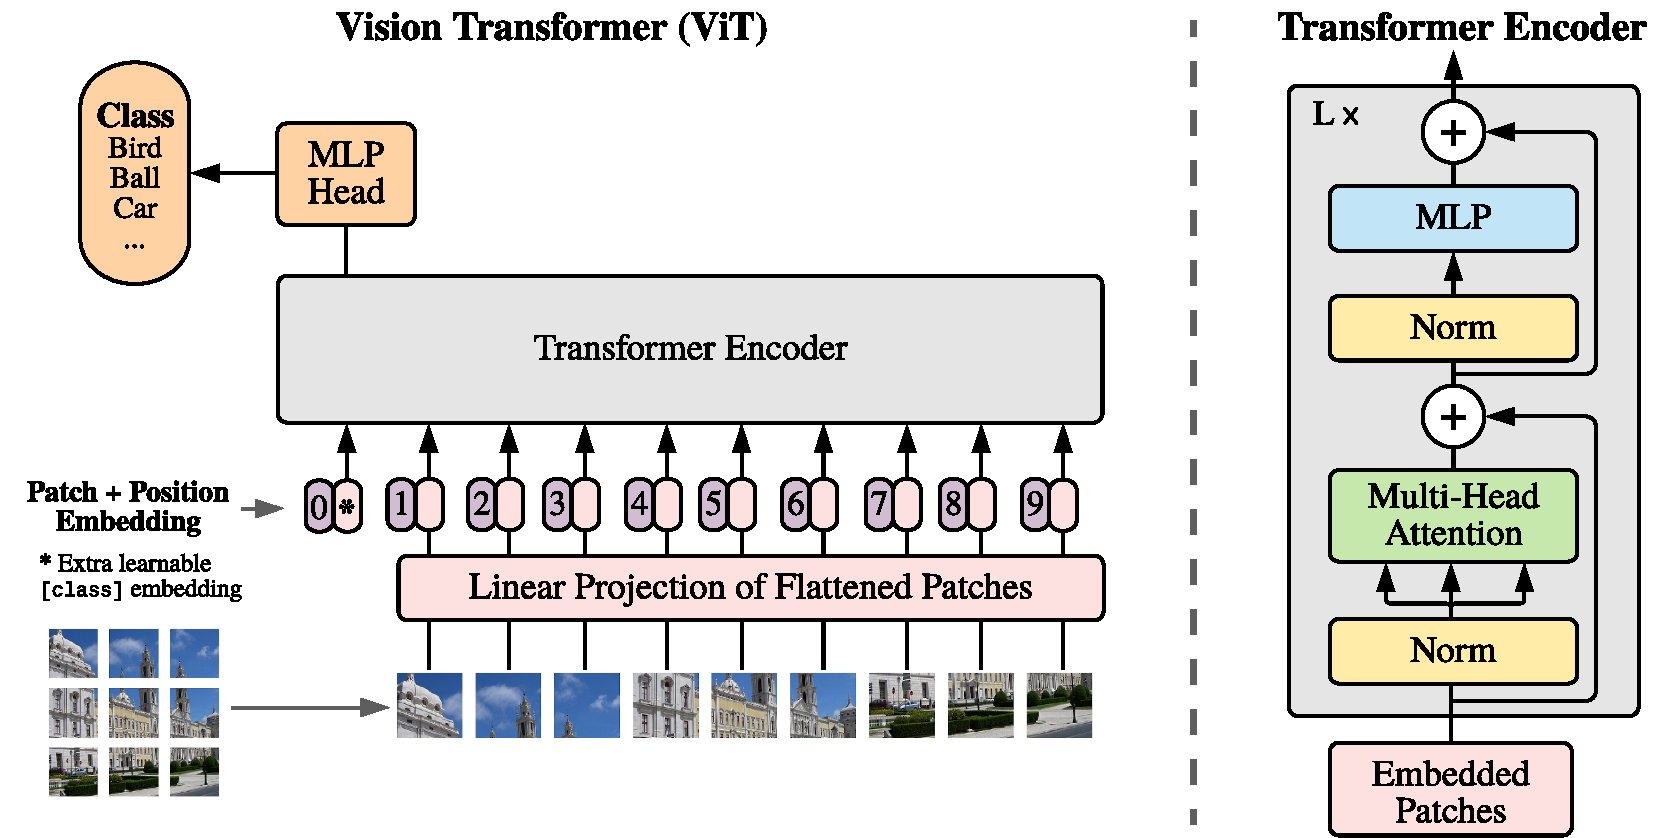
\includegraphics[width=0.95\linewidth]{pic/model_scheme}
        % \caption{We split an image into fixed-size patches, linearly embed each of them, add position embeddings, and feed the resulting sequence of vectors to a standard Transformer encoder. In order to perform classification, we use the standard approach of adding an extra learnable “classification token” to the sequence.}
        \label{fig:vit-figure}
    \end{figure}
\end{frame}



\begin{frame}{Patch Sizes}
    \begin{itemize}
        \item Patch size determines the granularity of the image representation.
        \item Smaller patches capture finer details but increase computational cost.
        \item The self-attention mechanism has $\mathcal{O}(N^2)$ complexity due to pairwise interactions between $N$ patches. 
        \item Larger patches reduce computational complexity but might miss finer details.
        \item In practice: 
            \begin{itemize}
                \item take 224x224 input image,
                \item divide it into a 16x16 grid of 14x14 pixel patches (or 14x14 grid of 16x16 patches)
            \end{itemize} 
        \item \textbf{An Image is Worth 16x16 Words!}
    \end{itemize}
\end{frame}


\begin{frame}{Positional Embeddings}
    \begin{itemize}
        \item We need to inject spatial information into the model to ensure the model understands the order of image patches.
        \item There are several options: 
        \begin{itemize}
            \item Providing no positional information: \textit{bag of patches}
            \item 1-dimensional positional embedding: sequence of patches in the raster order
            \item 2-dimensional positional embedding: concatenate embedding of different axes
            \item Relative positional embeddings: relative distance instead of absolute position
        \end{itemize}
        \item In practice 1-dimensional positional embedding work best.
    \end{itemize}
\end{frame}



\begin{frame}{Combining Patches and Embeddings}
    \begin{enumerate}
        \item \textbf{Divide Image into Patches}
        \begin{itemize}
            \item Image of size \( H \times W \) divided into patches of size \( P \times P \).
            \item Number of patches: \( N = \frac{H \times W}{P \times P} \).
        \end{itemize}
        \item \textbf{Flatten and Project Patches}
            \[
            \text{patch\_embedding}_i = \text{Linear}(\text{flatten}(x_i))
            \]
        \item \textbf{Add Positional Embeddings}
           \[
            \text{combined\_embedding}_i = \text{patch\_embedding}_i + PE_i
            \]
        \item \textbf{Form Input Sequence}
            \[
            \text{Input} = [\text{CLS}; \text{combined\_embedding}_1; \ldots; \text{combined\_embedding}_N]
            \]
    \end{enumerate}
\end{frame}


\begin{frame}{Transformer Encoder}
    \begin{itemize}
        \item Now that we have an \textbf{Input Sequence}, we can use a simple Transformer Encoder.
        \item A Transformer encoder consists of:
        \begin{itemize}
            \item  Multi-Head Attention: Learns relationships between all tokens (image patches) in the sequence.
        	\item Feedforward Network: Processes each token independently in a higher-dimensional space.
	        \item Residual Connections \& Layer Normalization: Helps with optimization.
        \end{itemize}
        \item Finally we can pass the output of the encoders to an MLP classifier head in order to predict the correct class.
    \end{itemize}
\end{frame}

\begin{frame}{Batch Normalization}
    \begin{columns}
        \begin{column}{0.65\linewidth}
        \begin{itemize}
            \item Normalizes inputs across the mini-batch.
            \[
            \hat{x}_{ij} = \frac{x_{ij} - \mu_{j}}{\sqrt{\sigma^2_{j} + \epsilon}}
            \]
            where \( \mu_{j} \) and \( \sigma^2_{j} \) are the mean and variance of the \( j \)-th feature in the mini-batch.
            \item Appropriate for CNNs.
            \item Requires large batch sizes.
            \item Improves generalization via regularization.
        \end{itemize}
        \end{column} 
        \begin{column}{0.4\linewidth} 
        \begin{figure}
            \centering
            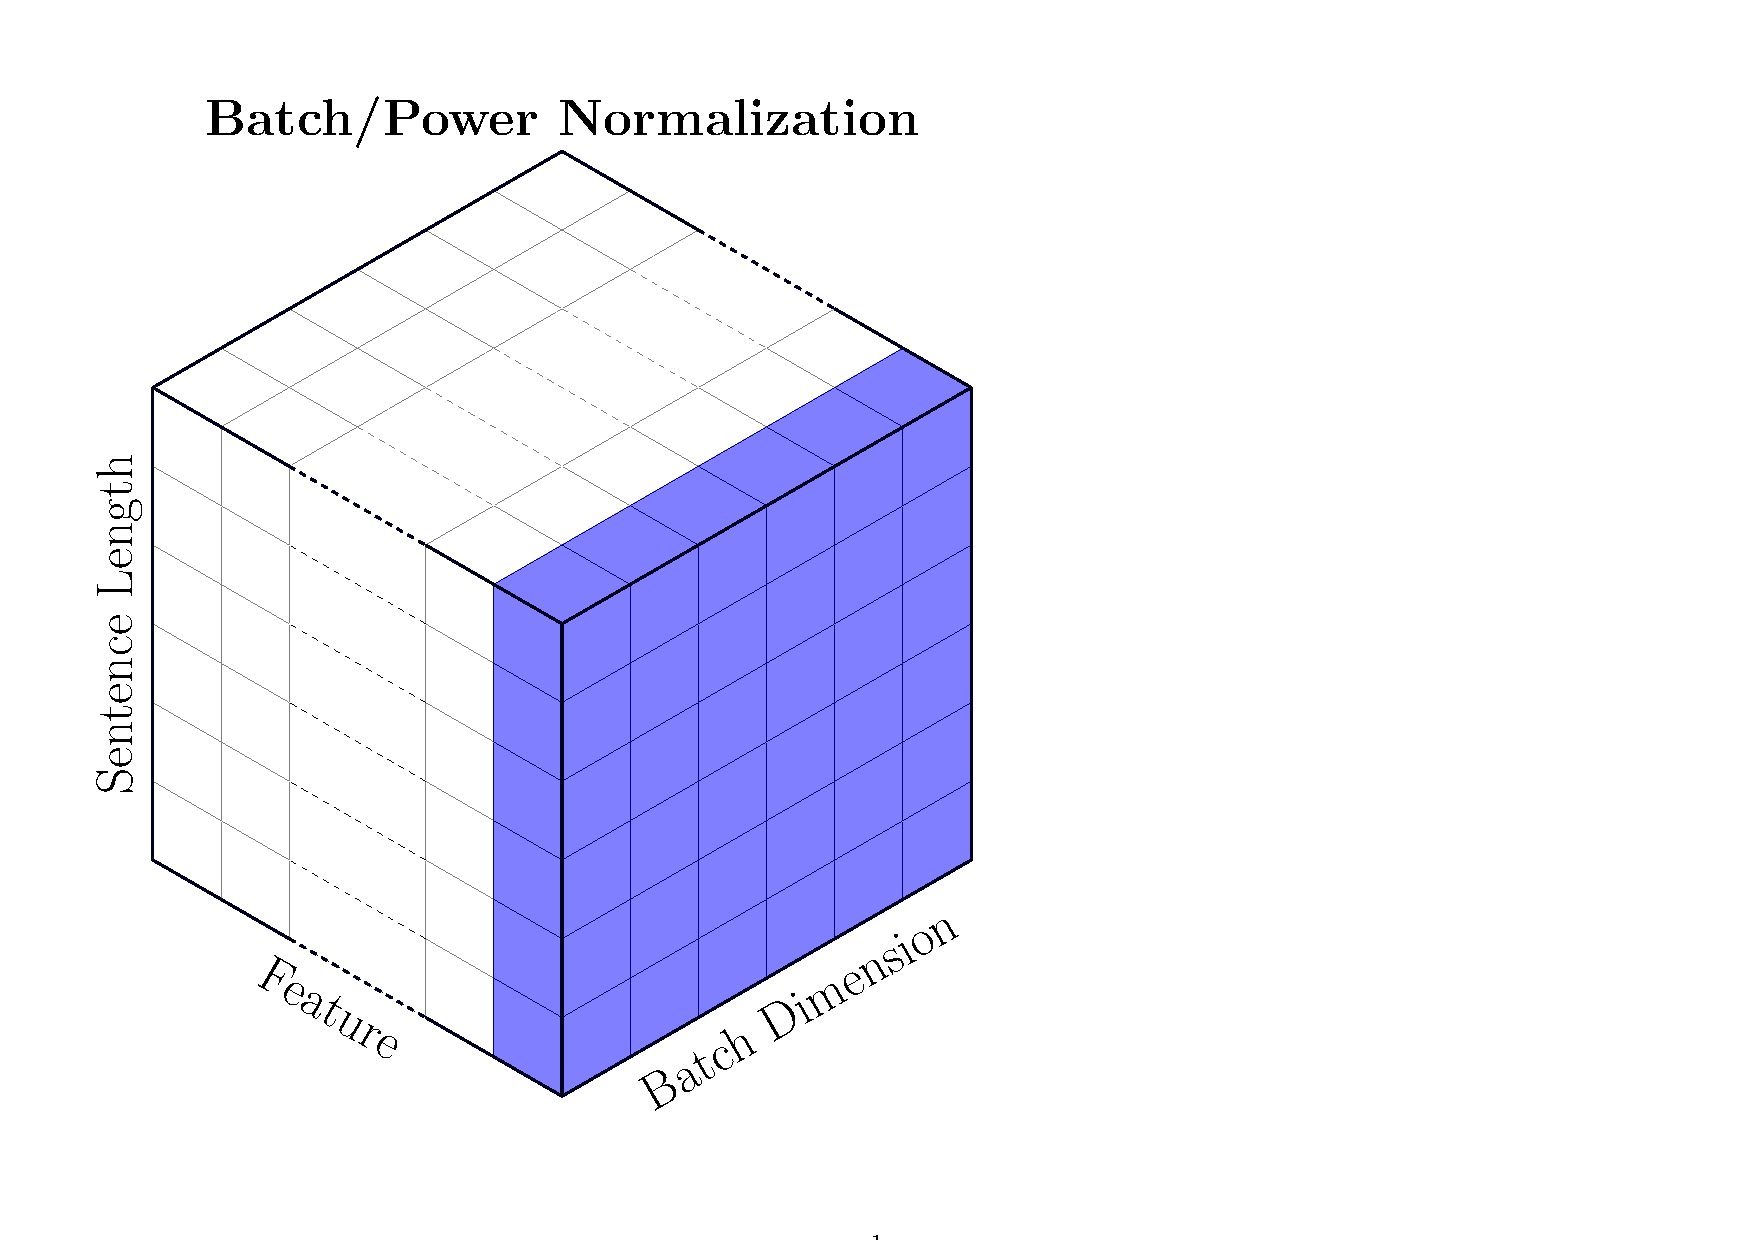
\includegraphics[width=1.5\linewidth]{pic/PN_vis.pdf}
            \label{fig:bn}
        \end{figure}
        \end{column}
    \end{columns}
\end{frame}

\begin{frame}{Layer Normalization}
    \begin{columns}
        \begin{column}{0.65\linewidth}
        \begin{itemize}
            \item Normalizes inputs across the features in a single training example.
            \[
            \hat{x}_{ij} = \frac{x_{ij} - \mu_{i}}{\sqrt{\sigma^2_{i} + \epsilon}}
            \]
            where \( \mu_{i} \) and \( \sigma^2_{i} \) are the mean and variance of the \( i \)-th training example.
            \item Appropriate for Transformers, RNNs, or NLP tasks.
            \item Works with small or dynamic batch sizes.
            \item Provides batch-independent normalization for flexibility.
        \end{itemize}
        \end{column} 
        \begin{column}{0.4\linewidth}
        \begin{figure}
            \centering
            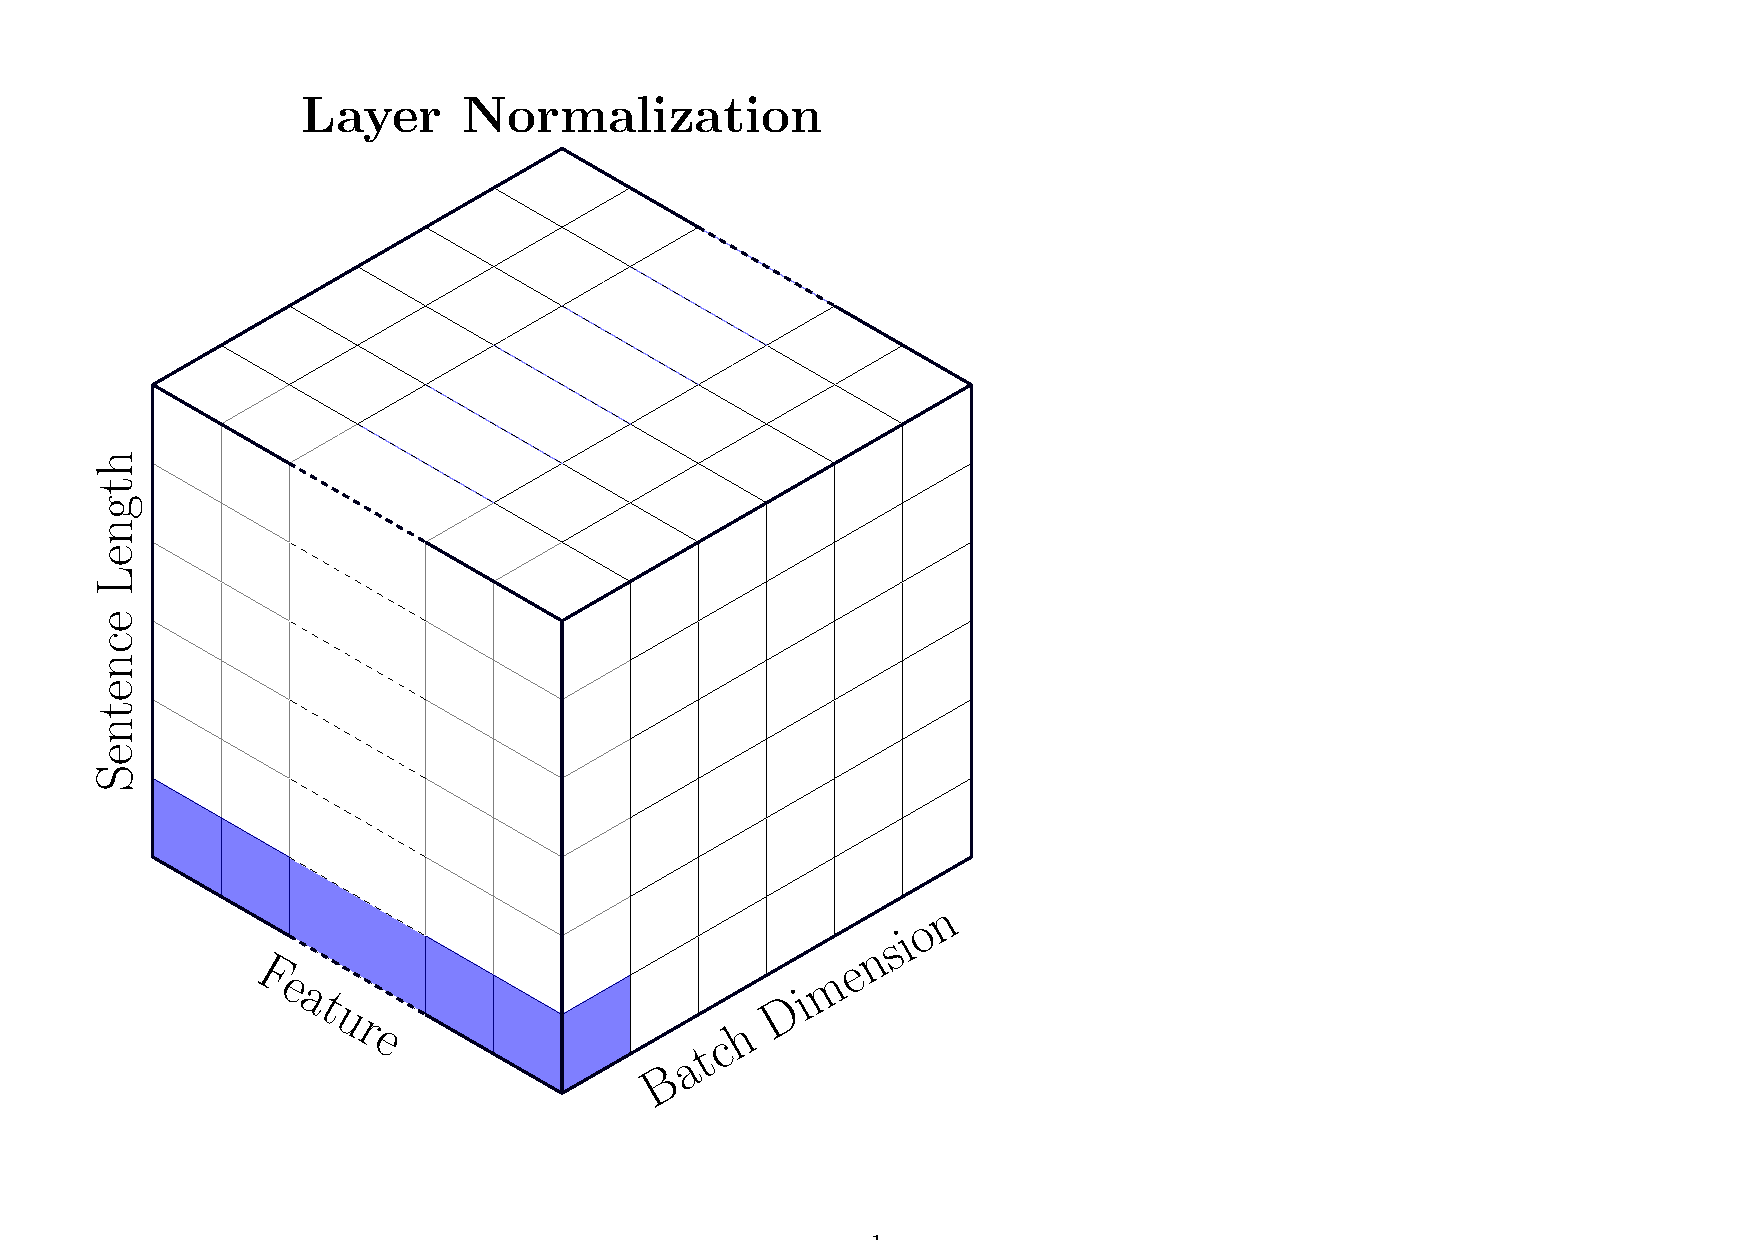
\includegraphics[width=1.5\linewidth]{pic/LN_vis.pdf}
            \label{fig:ln}
        \end{figure}
        \end{column}
    \end{columns}
\end{frame}

% \begin{frame}{Choosing The Right Normalization Scheme}
%     % \begin{tabular}{|p{2cm}|p{5cm}|p{5cm}|}
%     %     \hline
%     %     \textbf{Scheme} & \textbf{Advantages} & \textbf{Disadvantages} \\ \hline
%     %     \textbf{BatchNorm} & 
%     %     \begin{itemize}
%     %         \item Reduces internal covariate shift.
%     %         \item Acts as a regularizer.
%     %         \item Speeds up training.
%     %     \end{itemize} & 
%     %     \begin{itemize}
%     %         \item Depends on batch size.
%     %         \item Inefficient for small-batch or online learning.
%     %         \item Computational overhead.
%     %     \end{itemize} \\ \hline
%     %     \textbf{LayerNorm} & 
%     %     \begin{itemize}
%     %         \item Works with small batches.
%     %         \item Invariant to batch size.
%     %         \item Simple implementation.
%     %     \end{itemize} & 
%     %     \begin{itemize}
%     %         \item Less effective in CNNs.
%     %         \item Weaker regularization.
%     %     \end{itemize} \\ \hline
%     % \end{tabular}
% \end{frame}



\begin{frame}{What Do Positional Embeddings Learn?}
    \begin{columns}
        \begin{column}{0.6\textwidth}
            \begin{itemize}
                \item The model learns to encode distance within the image in the similarity of position embeddings.
                \item This means closer patches tend to have more similar position embeddings. 
                \item Patches in the same row/column have similar embeddings.
            \end{itemize}
        \end{column}
        \begin{column}{0.4\textwidth}
            \begin{figure}
                \centering
                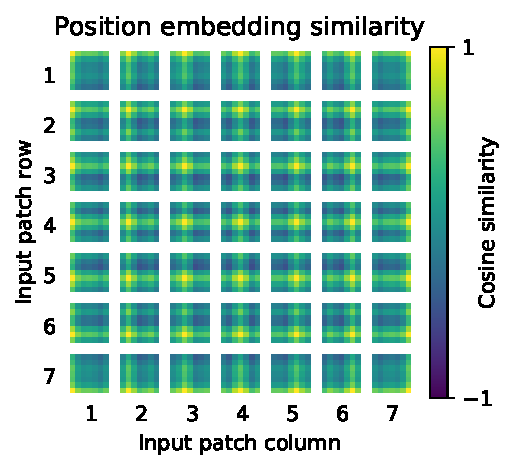
\includegraphics[width=\linewidth]{pic/20201002_position_embeddings_17085772_1.pdf}
                % \caption{Visualization of Positional Encodings}
                \label{fig:pos_encodings}
            \end{figure}
        \end{column}
    \end{columns}
\end{frame}

\begin{frame}{How Does Attention Help?}
    \begin{columns}
        \begin{column}{0.65\textwidth}
            \begin{itemize}
                \item Self-attention allows ViT to integrate information across the entire image even in the lowest layers.
                \item We can average attention weights across all heads and recursively multiply the weight matrices of all layers to mix attention across tokens through all layers.
            \end{itemize}
        \end{column}
        \begin{column}{0.35\textwidth}
            \begin{figure}
                \centering
                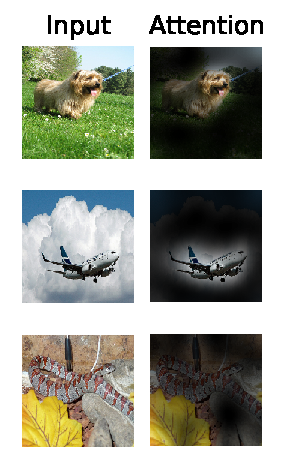
\includegraphics[width=0.8\textwidth]{pic/20201002_selected_attention_examples}
                % \caption{Representative examples of attention from the output token to the input space.}
                \label{fig:inspecting-vit}
            \end{figure}
        \end{column}
    \end{columns}
\end{frame}



\section{ViT vs. CNN}

\begin{frame}{Inductive Bias}
    \begin{itemize}
        \item In CNNs, locality, 2D neighborhood structure, and translation equivariance are baked into each layer throughout the whole model.
        \item In ViT, only MLP layers exhibit locality and translational equivariance, while self-attention layers capture global context.
        \item The 2D neighborhood structure is used very sparingly.
    \end{itemize}
\end{frame}

\begin{frame}{Combining CNNs and Transformers}
    \begin{itemize}
        \item As an alternative to raw image patches, the input sequence can be formed from feature maps of a CNN.
	    \item These hybrid models combine the local feature extraction capabilities of CNNs with the global context awareness of Transformers. 
        \item These models can perform well even on smaller datasets.
    \end{itemize}
\end{frame}

\begin{frame}{Dataset Size}
    \begin{columns}
        \begin{column}{0.5\textwidth}
            \begin{figure}
                \centering
                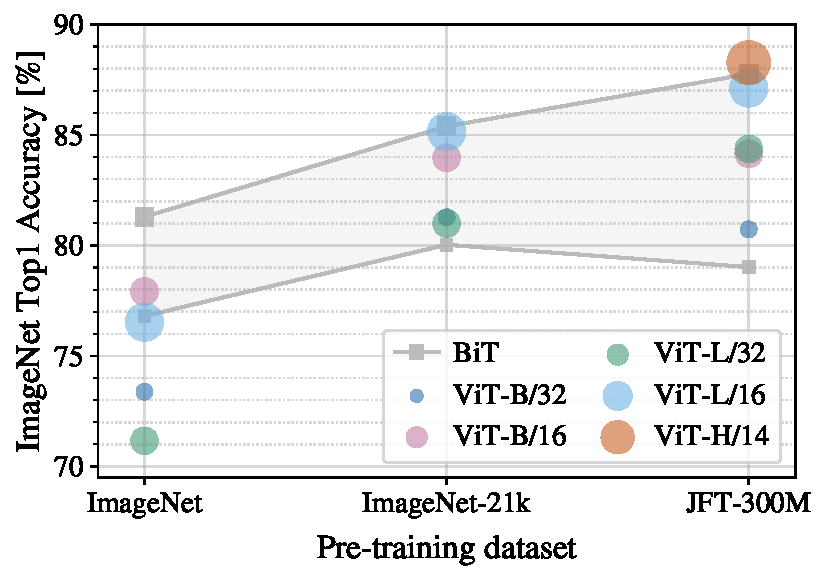
\includegraphics[width=\textwidth]{pic/transvolution-i1k-scaling}
                % \caption{
                % % Transfer to ImageNet. 
                % While large ViT models perform worse than BiT ResNets when pre-trained on small datasets, they shine when pre-trained on larger datasets. 
                % %Similarly, larger ViT variants overtake smaller ones as the dataset grows.
                % }
                \label{fig:transvolution}
            \end{figure}
        \end{column}
        \begin{column}{0.5\textwidth}
            \begin{figure}
                \centering
                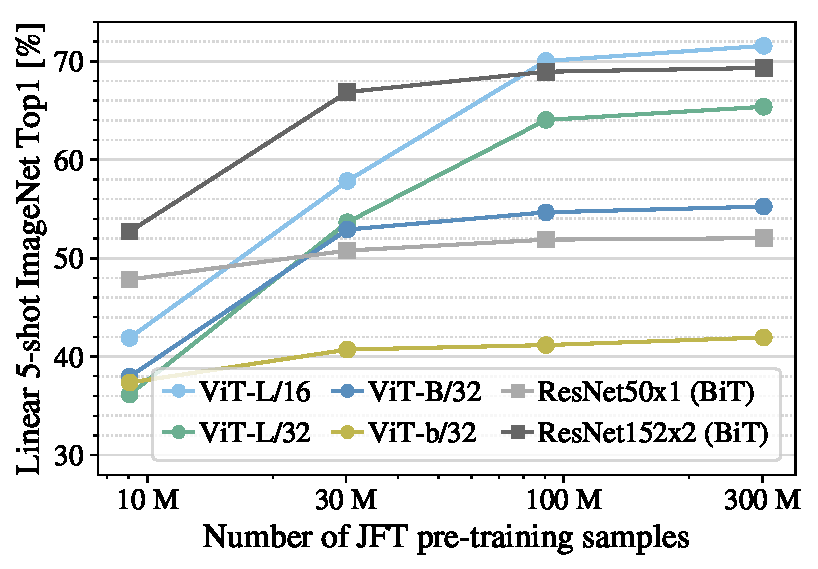
\includegraphics[width=\textwidth]{pic/imagenet_5shot}
                % \caption{
                % % Linear few-shot evaluation on ImageNet versus pre-training size. 
                % ResNets perform better with smaller pre-training datasets but plateau sooner than ViT, which performs better with larger pre-training. 
                % %ViT-b is ViT-B with all hidden dimensions halved.
                % }
                \label{fig:imagenet_5shot}
            \end{figure}
        \end{column}
    \end{columns}
\end{frame}


\begin{frame}{Performance vs. Pre-training}
    \begin{figure}
        \centering
        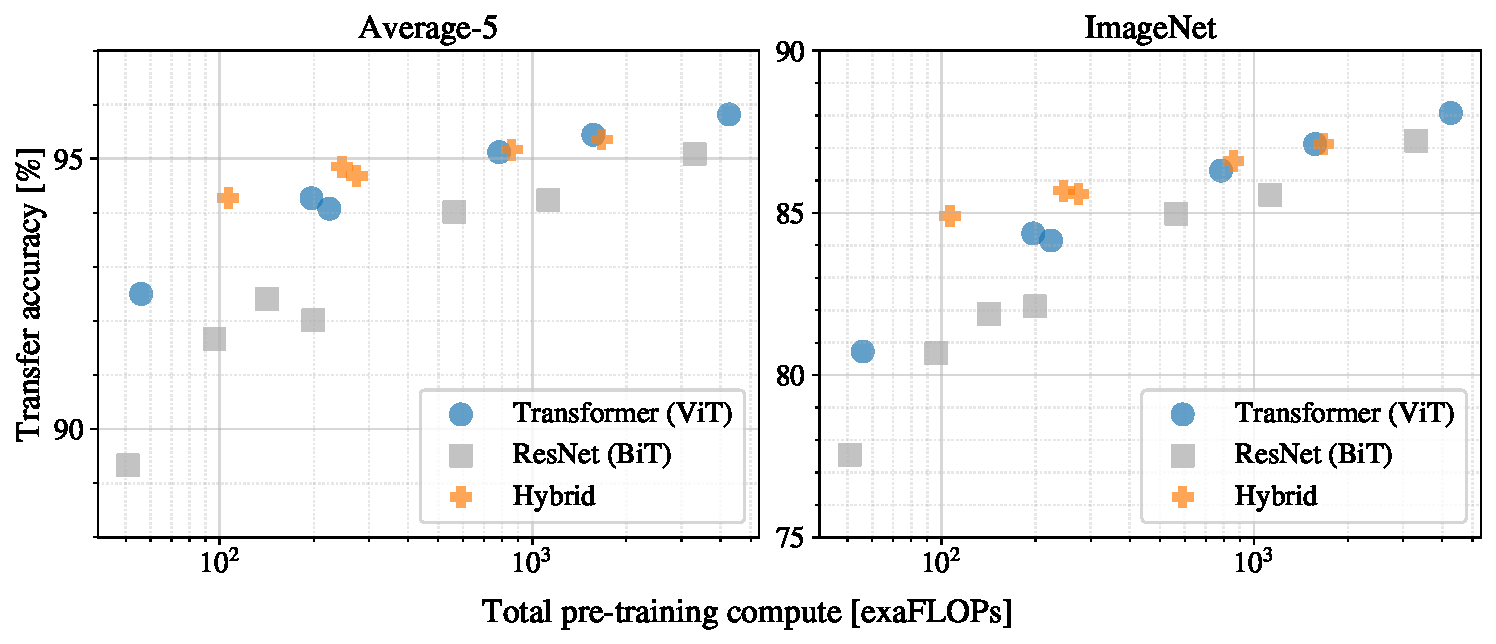
\includegraphics[width=0.9\linewidth]{pic/finetune_vs_compute2.pdf}
        % \caption{Vision Transformers generally outperform ResNets with the same computational budget. Hybrids improve upon pure Transformers for smaller model sizes, but the gap vanishes for larger models.}
        \label{fig:enter-label}
    \end{figure}
\end{frame}


\begin{frame}{State-of-the-Art}
    \begin{itemize}
        \item Transformers achieve State-of-the-Art results in a variety of computer vision tasks, including \textbf{Classification}, \textbf{Segmentation}, \textbf{Detection}, and more!
    \end{itemize}
    \begin{figure}
        \centering
        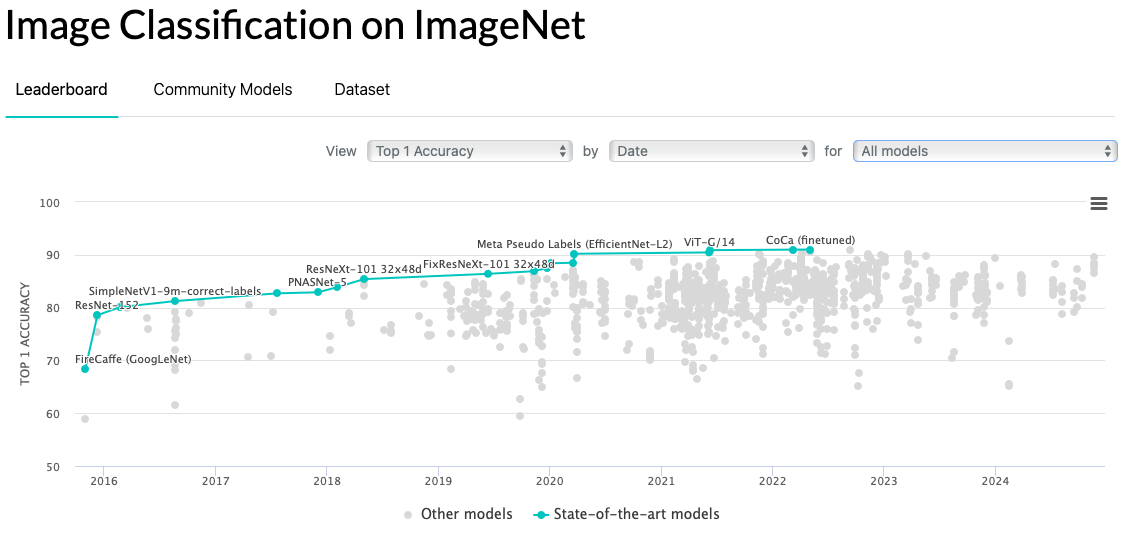
\includegraphics[width=\linewidth]{pic/SOTA.png}
        % \caption{State-of-the-Art Performance}
        \label{fig:sota}
    \end{figure}
\end{frame}

\begin{frame}{Conclusion}
    \begin{itemize}
        \item \textbf{Advantages of ViTs}
        \begin{itemize}
            \item \textbf{Better with Scale}: Performance improves significantly as dataset size and model size grow.
            \item \textbf{Unified Architecture}: The same Transformer blocks can be applied to text, images, and other modalities.
            \item \textbf{Interpretability}: Attention maps can provide insights into which patches are influencing the final decision.
        \end{itemize}
        \item \textbf{Disadvantages of ViTs}
        \begin{itemize}
            \item \textbf{Data Hungry}: ViTs typically require large pretraining datasets.
            \item \textbf{Computational Cost}: Multi-head self-attention scales quadratically with the number of tokens. For high-resolution images, this can be expensive.
            \item \textbf{Overfitting}: High capacity can lead to overfitting.
        \end{itemize}
    \end{itemize}
\end{frame}



\section{References}

\begin{frame}{Contributions}
    \begin{itemize}
        \item These slides have been prepared thanks to: 
	    \begin{itemize}
	        \item Ramtin Moslemi
	    \end{itemize}
    \end{itemize}
\end{frame}


\begin{frame}{References}
    \bibliography{ref}
    \bibliographystyle{ieeetr}
    \nocite{*}
\end{frame}

\end{document}